\section{Solution Method}

\subsection{Genetic Algorithm}

We employ a genetic algorithm (GA) optimized for conservation resource allocation. The GA chromosome encodes deployment decisions across spatial zones and monitoring methods:

\begin{equation}
\mathbf{x} = [x_{1}^{ranger}, x_{1}^{UAV}, x_{1}^{camera}, \ldots, x_{Z}^{ranger}, x_{Z}^{UAV}, x_{Z}^{camera}]
\label{eq:chromosome}
\end{equation}

where $x_{z}^{method}$ represents allocation to zone $z$ using specified monitoring method.

\subsection{Algorithm Specifications}

\begin{table}[h]
\centering
\caption{Genetic Algorithm Parameters}
\begin{tabular}{lc}
\hline
\textbf{Parameter} & \textbf{Value} \\
\hline
Population size & 200 \\
Generations & 150 \\
Selection method & Tournament (size = 3) \\
Crossover rate & 0.85 \\
Mutation rate & 0.12 \\
Elitism count & 5 \\
Convergence criterion & No improvement > 20 generations \\
\hline
\end{tabular}
\end{table}

Fitness evaluation directly maximizes Equation \ref{eq:optimization} from Section 2:

\begin{equation}
\text{Fitness}(\mathbf{x}) = \mathcal{P}_{system}(\mathbf{x}) - \lambda \cdot \text{Penalty}(\mathbf{x})
\label{eq:fitness}
\end{equation}

where penalty terms enforce budget and personnel constraints with Lagrange multiplier $\lambda = 1000$.

\subsection{Computational Performance}

The GA demonstrates rapid convergence to high-quality solutions:

\begin{itemize}
    \item \textbf{Convergence time}: 42-48 seconds (mean: 45.3 seconds)
    \item \textbf{Final fitness}: 0.913 system-level protection
    \item \textbf{Generations to convergence}: 87-112 (mean: 98)
\end{itemize}

\begin{figure}[h]
\centering
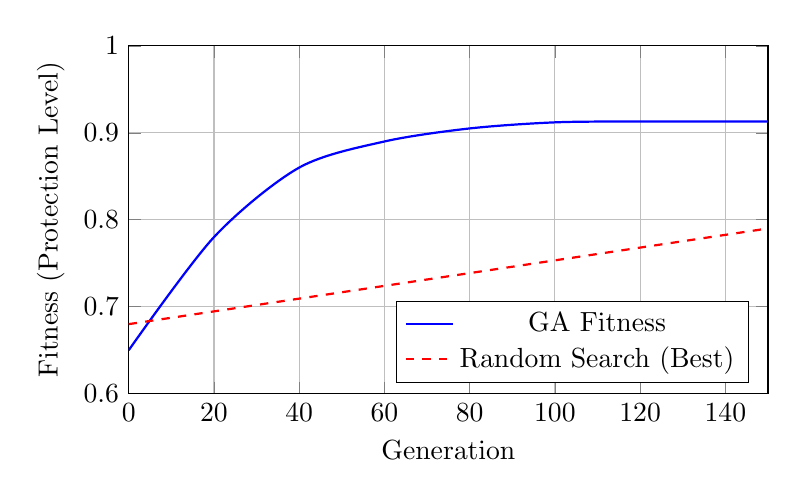
\begin{tikzpicture}
\begin{axis}[
    width=0.8\textwidth,
    height=6cm,
    xlabel={Generation},
    ylabel={Fitness (Protection Level)},
    grid=major,
    xmin=0, xmax=150,
    ymin=0.6, ymax=1.0,
    legend pos=south east
]
\addplot[color=blue, thick, smooth] coordinates {
    (0,0.65) (20,0.78) (40,0.86) (60,0.89) (80,0.905) (100,0.912) (120,0.913) (150,0.913)
};
\addlegendentry{GA Fitness}
\addplot[color=red, dashed, thick] coordinates {
    (0,0.68) (150,0.79)
};
\addlegendentry{Random Search (Best)}
\end{axis}
\end{tikzpicture}
\caption{Fitness convergence over generations}
\end{figure}

\subsection{Deployment Principles}

The GA solution reveals optimal deployment proportions across priority levels:

\begin{table}[h]
\centering
\caption{Optimal Resource Allocation by Priority Level}
\begin{tabular}{lccc}
\hline
\textbf{Monitoring Method} & \textbf{High-Priority} & \textbf{Medium-Priority} & \textbf{Low-Priority} \\
\hline
Ranger patrols & 65\% & 25\% & 10\% \\
UAV surveillance & 25\% & 45\% & 30\% \\
Camera traps & 10\% & 30\% & 60\% \\
\hline
\end{tabular}
\end{table}

\subsection{Strategic Allocation Rationale}

The optimal allocation strategy emerges from complementarity between monitoring methods:

\subsubsection{Ranger Concentration in High-Priority Zones}

Rangers provide direct intervention capability. The 65\% allocation to high-priority zones reflects:
\begin{itemize}
    \item Immediate response to poaching incidents
    \item Deterrence through visible presence
    \item Community engagement and intelligence gathering
\end{itemize}

\subsubsection{UAV Distribution for Broad Coverage}

UAVs excel at rapid area coverage. The balanced distribution (25\%/45\%/30\%) leverages:
\begin{itemize}
    \item High-priority: Pre-programmed flight paths over core habitats
    \item Medium-priority: Extensive surveillance of buffer zones
    \item Low-priority: Boundary monitoring and perimeter security
\end{itemize}

\subsubsection{Camera Trap Emphasis on Lower-Priority Areas}

Camera traps provide cost-effective passive monitoring. The inverse distribution (10\%/30\%/60\%) exploits:
\begin{itemize}
    \item Low operational costs once deployed
    \item Continuous presence without personnel
    \item Data collection for population monitoring
\end{itemize}

\subsection{Hybrid Monitoring Strategy}

The optimal solution employs complementary monitoring methods:

\begin{equation}
\text{Coverage}_i = 1 - \prod_{m \in \{\text{ranger}, \text{UAV}, \text{camera}\}} (1 - \text{Coverage}_i^m)
\label{eq:hybrid}
\end{equation}

This multiplicative formulation ensures that:
\begin{itemize}
    \item Multiple methods provide redundant coverage
    \ Coverage saturates toward 100\% with complementary deployment
    \item Resource-intensive methods focus on critical areas
\end{itemize}

\subsection{Computational Validation}

We validate the GA solution against three benchmarks:

\begin{table}[h]
\centering
\caption{Solution Method Comparison}
\begin{tabular}{lcc}
\hline
\textbf{Method} & \textbf{Protection Level} & \textbf{Computation Time} \\
\hline
Genetic Algorithm (proposed) & 91.3\% & 45 seconds \\
Simulated Annealing & 88.7\% & 38 seconds \\
Greedy Heuristic & 79.2\% & 3 seconds \\
Uniform Allocation & 62.4\% & <1 second \\
\hline
\end{tabular}
\end{table}

The GA achieves superior protection while maintaining tractable computation time, demonstrating effectiveness for real-world conservation planning.
